\chapter{Výsledky studentské práce}

% Referenční skladby http://isophonics.net/about

\section{Návrh výsledného systému}

Návrh popisuje komplexní systém skládající se z několika částí, uživatelské rozhraní, algoritmů pro získání pamrametrů hudební nahrávky a algoritmu generujícího SpectodaCode na základě získaných parametrů. V této kapitole je podrobně popsán návrh jednotlivých částí systému. 

\subsection{Uživatelské rozhraní} \label{sec:User_interface}

Uživatelské rozhraní je reprezentováno webovou stránkou a je naprogramováno pomocí značkovacího jazyka \acs{HTML} spolu s formátováním v jazyce CSS. Funkčnost webové stránky je zajištěna funkcemi v jazyce JavaScript. Javascript také tvoří propojovací můstek pro komunikaci s vnitřním systémem v jazyce Python.

Jedná se o jednoduché webové rozhraní, ve kterém uživatel nahraje hudební skladbu ve formátu .wav. Rozhranní obsahuje pole pro vložení cesty k hudební skladbě umožňující výběr ze souborů v uživatelově uložišti. Níže je posuvník s 4 základními hodnotami pro výběr nálady
\uv{mood}. Jedná se hodnoty \uv{chill}, \uv{hang out}, \uv{feeling happy} a \uv{dancing}, které jsou v tomto pořadí na posuvníku. Uživatel může pomocí posouvání posuvníku vybrat pro jakou náladu chce vytvořit animaci. Pod posuvníkem pro výběr nálady se nachází tlačítko spouštějící proces generování SpectodaCodu.
Poslední částí webového rozhraní je textové pole ve kterém se zobrazí vygenerovaný SpectodaCode. Na blokovém schématu \ref{fig:User_interaction_diagram} je zobrazen proces postupu uživatele skrze webové rozhraní. 

 \begin{figure}[H]
    \centering
    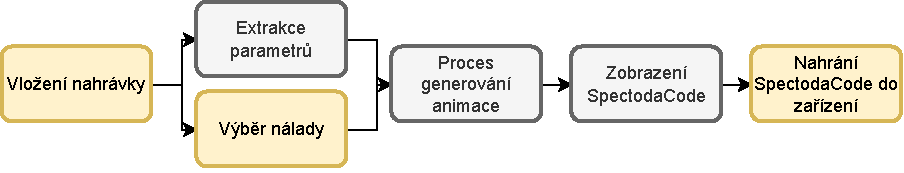
\includegraphics[width = 1\linewidth]{obrazky/User_interaction_diagram.pdf}
    \caption{Blokové schéma postupu uživatele webovou stránkou}
    \label{fig:User_interaction_diagram}
\end{figure}

\subsection{Parametry hudební nahrávky} \label{sec:Parametry_nahravky}

Systém popsaný v bodě \ref{sec:System_generovani_animaci} vyžaduje vstupní data o hudební nahrávce. Tyto data jsou rozdělena na 7 parametrů. Každý z parametrů představuje vlastnost analyzované nahrávky. Tyto vlastnosti jsou získány pomocí technik popsaných v bodě \ref{sec:Exktrakce_vlastnosti_metody}. Jednotlivé vlastnosti a jejich datové struktury jsou shrnuty v následujících bodech.

\begin{description}
    \item[Detekce dob] představuje pole hodnot jehož délka je závislá na době trvání nahrávky. Jednotlivé hodnoty pak udávají časy hudební nahrávky, ve kterých se nacházejí doby.
    \item[Tempo skladby] je číslo typu float s jednotkou \acs{BPM} vyjadřující počet úderů za minutu. Hodnota BPM se vztahuje k počtu čtvrťových not za minutu. Vybraný algoritmus z knihovny Librosa ovšem nedetekuje jestli se jedná o noty čtvrťové. Postup zjištění tempa je popsán v bodě \ref{sec:Librosa}.
    \item[Chromavektory] jsou získány v podobě pole jehož počet řádků udává 12 půltónů rozdělujících 1 oktávu. Délka pole je závislá na délce nahrávky a velikosti okna  při výpočtu \acs{STFT}. K matici chromavektorů je přidáno pole o stejné délce. Hondonty v poli udávají čas konce okna, ve kterém jsou počítány chroma vlastonsti. Tyto dvě proměnné jsou zadány jako parametry třídy s názvem \textit{ChromaVector} jehož struktura je zobrazena v blokovém schématu \ref{fig:ChromaVector_class_diagram}.

    \begin{figure}[H]
        \centering
        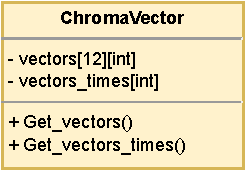
\includegraphics[width = 0.3\linewidth]{obrazky/UML_diagram_ChromaVector.pdf}
        \caption{Struktura třídy \textit{ChromaVector}}
        \label{fig:ChromaVector_class_diagram}
    \end{figure}

    \item[Efektivní hodnota signálu] je zapsána třídou $Loudness$ obsahující dva atributy. Prvním z nich je pole $rms$ jehož délka je závislá na délce signálu a obsahuje efektivní hodnoty signálu v časech uložených v druhém atributu $times$.
    
    \begin{figure}[H]
        \centering
        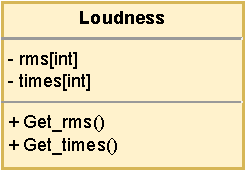
\includegraphics[width = 0.3\linewidth]{obrazky/UML_diagram_Loudness.pdf}
        \caption{Struktura třídy $Loudness$}
        \label{fig:Loudness_class_diagram}
    \end{figure}

    \item[Segmentace] je zapsána jako pole objektů tířdy $Segment$. Tato třída obshahuje 3 atributy $type$, $start\_time$ a $end\_time$. Proměnná $type$ obsahuje statickou hodnotu označující o jakou část skladby se jedná. Tyto hodnoty jsou vypsány v úryvku kódu \ref{code:song_segments_variables}.
    Proměnné $start\_time$ a $end\_time$ označují začátek a konec segmentu v nahrávce. 

    \begin{figure}[H]
        \centering
        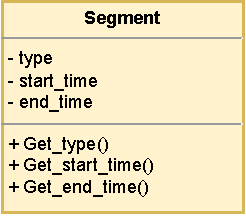
\includegraphics[width = 0.3\linewidth]{obrazky/UML_diagram_Segment.pdf}
        \caption{Struktura třídy $Segment$}
        \label{fig:Loudness_Segment_diagram}
    \end{figure}
    \begin{lstlisting} [
        caption = {Hodnoty proměnné $type$},
        captionpos=b,
        label = {code:song_segments_variables}]
        # Song segments variables
        SILENT      = 0
        REFRAIN     = 1
        STROPHE     = 2
        BRIDGE      = 3
    \end{lstlisting}

    \item[Žánr] představuje proměnou $genre$ typu short ve které je zapsáno číslo označující žánr skladby. Statické hodnoty žánrů jsou zapsány v úryvku kódu \ref{code:song_genre_variables}.
    \begin{lstlisting} [
        caption = {Hodnoty proměnné $genre$},
        captionpos=b,
        label = {code:song_genre_variables}]
        # Song genre variables
        CLASSIC     = 0
        FOLK        = 1
        POP         = 2
        ROCK        = 3
        METAL       = 4
        ELECTRONIC  = 5
    \end{lstlisting}
    \item[Nálada] představuje proměnou $mood$ typu float s přednastavenými statickými hodnotami zobrazenými v části kódu \ref{code:song_mood_variables}. Nálada může být i v rozmezí přednastavencýh hodnot. V tomto případě je výsledná hodnota lineráně závislá na vzdálenosti od přednastavených hodnot. 
    \begin{lstlisting}[
        caption = {Hodnoty proměnné $mood$},
        captionpos=b,
        label = {code:song_mood_variables}]
        # Song mood variables
        CHILL       = 0
        HANG_OUT    = 1
        HAPPY       = 2
        DANCING     = 3
    \end{lstlisting}
    
\end{description}

\subsection{Systém pro generování animací} \label{sec:System_generovani_animaci}

Systém pro generování animací je jádrem práce. Jeho struktura udává vizuální kvalitu animací a schopnost přizpůsobit se žánrově různorodým skladbám. V této kapitole je popsána struktura systému. 

První částí systému je vstupní rozhraní, ve kterém jsou přijímány data obsahující paramery o hudební nahrávce. Struktura přijímaných dat je popsána v budě \ref{sec:Parametry_nahravky}. Každý ze zmíněných parametrů plňí důležitou funkci v rozhodovacím procesu skládání bloků animace. Níže jsou popsány rozhodovací funkce pro jednotlivé parametry.

\begin{description}
    \item[Žánr a nálada] jsou používány pro výběr vhodného balíčku animací. Tyto balíčky jsou nazývány datasety a jejich datová struktu je popsána v bodě \ref{sec:Database_structure}. Źánr i nálada jsou zaznamenány jako předdefinovaná celočíslená hodnota. Postup výběru datasetu je následující. Každý dataset obsahuje seznam žánrů pro který je vhodný. Na základě proměnné $genre$ dochází k výběru všech datasetů vhodných pro daný žánr. Následně na základě proměnné $mood$ ve které je uložená nálada je vybráno 5 datasetů s nejbližší hodnotou $mood\_characteristic$.
    
    \begin{figure}[H]
        \centering
        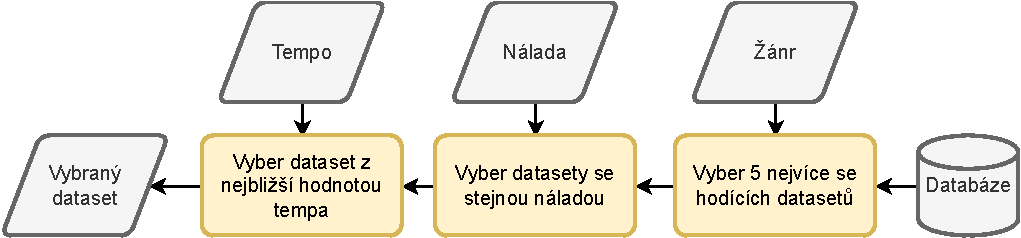
\includegraphics[width = 1\linewidth]{obrazky/Dataset_selection_diagram.pdf}
        \caption{Blokový diagram výběru datasetu.}
        \label{fig:Dataset_selection_diagram}
    \end{figure}

    \item[Tempo skladby] je posledním parametrem při výběru vhodného datasetu. 
    Hodnota proměnné \textit{speed\_suitability} každého z 5 vybraných datasetů je porovnána s tempem skladby. Finální dataset je vybrán ten jehož hodnota \textit{speed\_suitability} je nejbližší hodnotě tempa skladby. Blokový diagram procesu je znázoprněn na obrázku \ref{fig:Dataset_selection_diagram}. Tempo skladby je také použito pro výpočet délky jednotlivých animací na které je přímo úměrná rychlost animace.
    \item[Segmentace] slouží pro detekci opakujících se částí nahrávky. Například nahrávka obsahuje více než jednu sloku či refrém. Je kladen důraz aby v opakujících se segmentec nahrávky byla animace stejného typu. Z toho plyne, že v každém refrému bude podobná animace.
    \item[Detekce dob] je parametrem na základě kterého se nastaví začátky a konce animací tak, aby odpovídaly rytmu nahrávky.
    \item[Chroma vektory] udávají tónovou strukturu skladby v průběhu času. Tento parametr je využit pro nastavení barevné škály animací. Chromavektory se analyzují a jsou vybrány 4 hlavní tóny nejčastěji se vyskytující v nahrávce. Keždému tónu je přiřazen barevný odstín. Poté je animaci v dané části skladby přiřazena barva dle tónu určeného chromavektorem daného času nahrávky.
    \item[Efektivní hodnota signálu] pomáha procesu segmentace. Refrém a sloka se mohou lyšit hlasitostí, která je zpjata s efektní hodnotou. Zároveň je použita pro výběr vhodného typu animace. Na základě velikosti efektivní hodnoty signálu v čase je vybrán typ animace. Vyžší hodnoty představují rychlejší a údernější animace. Nižší hodnoty naopak pomalejší a klidnější animace. Tento proces je zajištěn porovnáváním proměnné \textit{anim\_characteristic} obsažené v každém bloku animace s efektivní hodnotou mapovanou na určený rozsah.
    %TODO: Vymyslet a pospat proces mapování efektivní hodnoty. 
    %TODO: Popsat tak aby to odpovídalo struktuře anim_characteristic dle blokového diagramu.
\end{description}

\
Druhá část systému tvoří samotnou logiku skládání blkoků animací. Tato rozhodovací struktura je zobrazena na blokovém diagramu \ref{fig:Logical_structure_diagram}.

\begin{figure}[H]
    \centering
    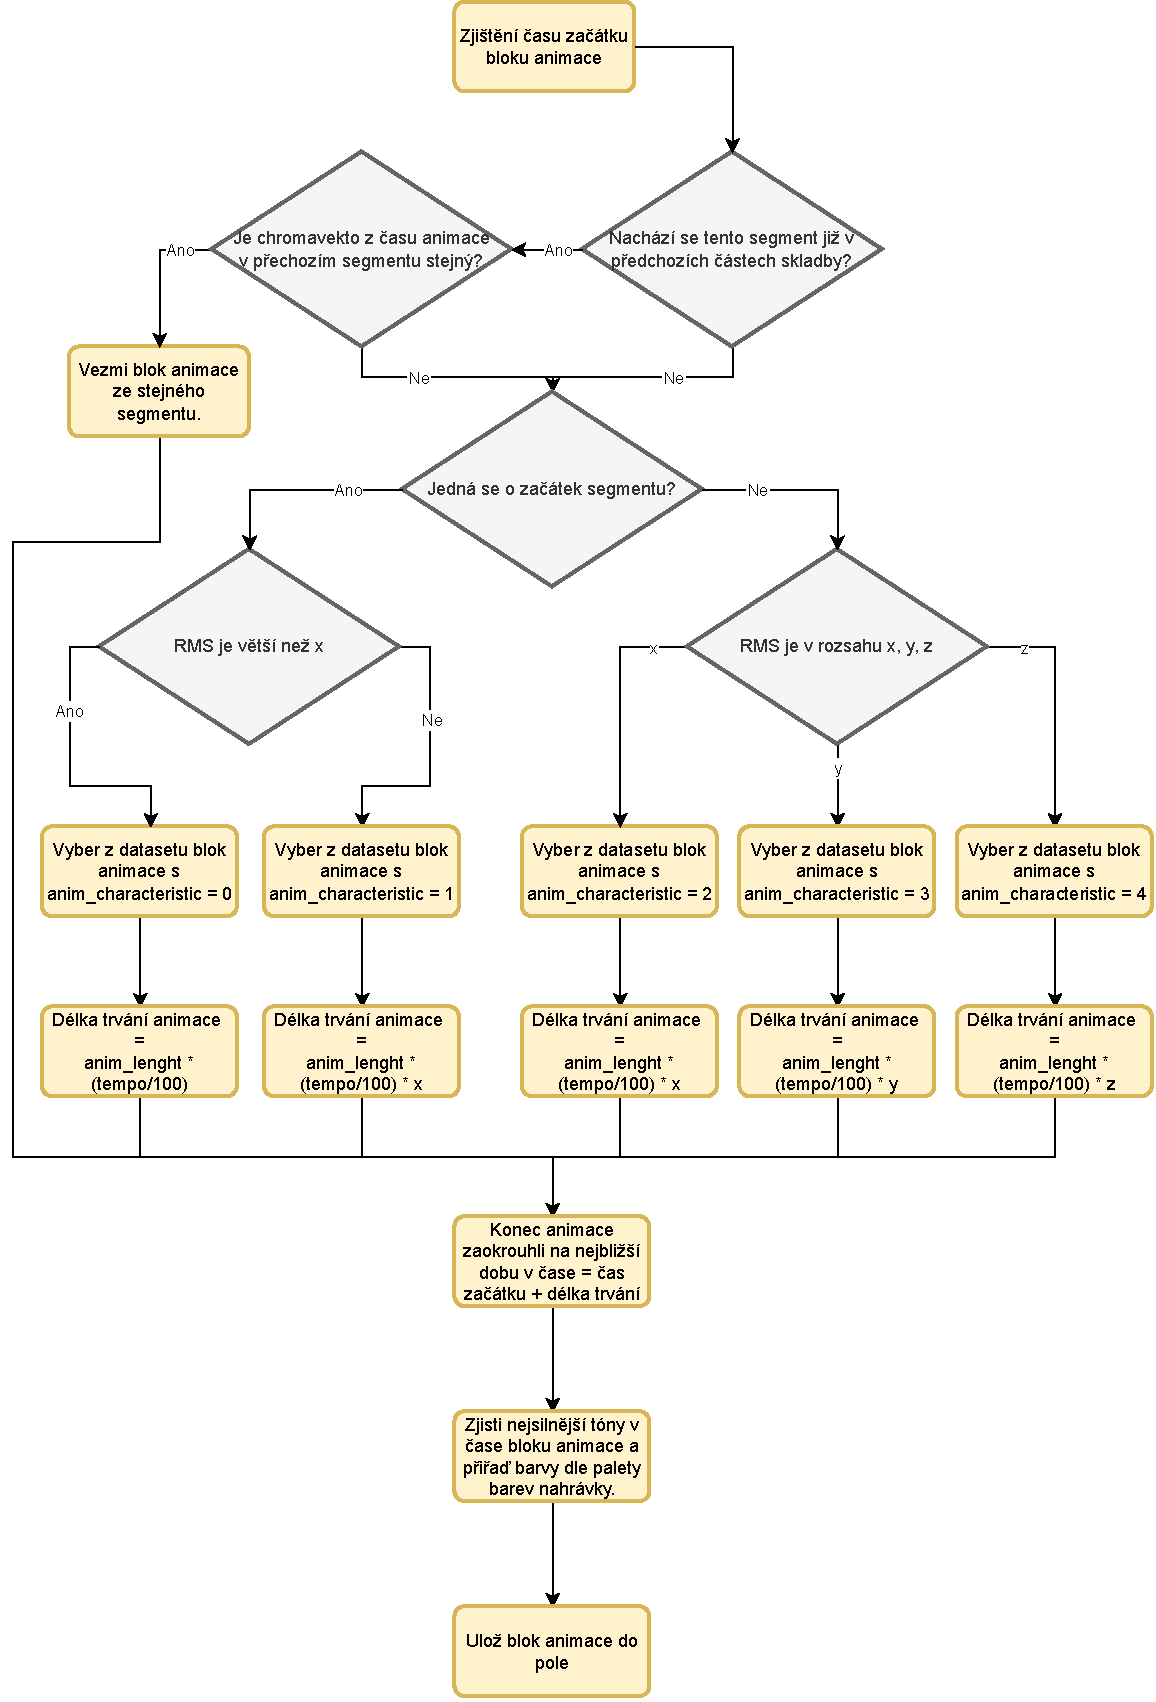
\includegraphics[width = 1\linewidth]{obrazky/Logical_structure_diagram.pdf}
    \caption{Blokový diagram struktrury rozhodovacího procesu}
    \label{fig:Logical_structure_diagram}
\end{figure}

% Na začátku je zjištěno jestli se jedná o první blok animace. Pokud ano je nastaven čas začátku animace jako čas první doby v nahrávce. Jestli se nejedná o první blok animace, tak je nastaven čas začátku jako konec předchozího bloku animace. Tento proces v blokovém schématu \ref{} představuje proces s názvem \uv{Nastavení času začátku animace}. Druhým krokem je rozhodovací struktura jestli se vybraný čas začátku nachází v segmentu nahrávky který se opakuje. Pokud ano je nalezen blok animace ve stejném času předchozího segmentu a je zkontrolováno  


\subsection{Databáze bloků animací} \label{sec:Database_structure}
Jak je popsáno v bodě \ref{sec:Spectoda} systém Spectoda obsahuje základní animace, které jsou skládány dosebe a tím vznikají komplexní animace. Navržený systém využívá již návrhářem předsložených animací, které jsou uloženy jako bloky. Těmto blokům jsou přiřazeny parametry $code$, $characteristic$ a $length$. Jejich struktura je zapsaná datovou třídou $AnimationBlock$.
Z objektů tipu \textit{AnimationBlock} jsou dále tvořeny datasety zapsané datovou třídou \textit{Dataset}. Tyto datasety obsahují 5 bloků animací a parametry \textit{genre}, \textit{speed\_suitability} a \textit{mood\_characteristic}. UML diagramy tříd jsou zobrazeny na obrázku \ref{fig:UML_diagram_Dataset_AnimationBlock}.

\begin{figure}[H]
    \centering
    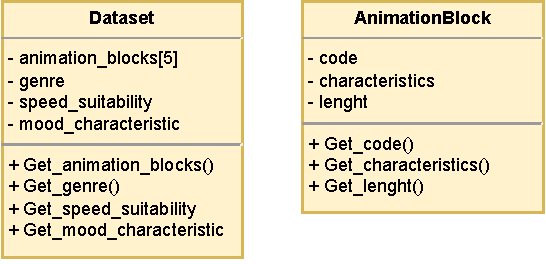
\includegraphics[width = 0.7\linewidth]{obrazky/UML_diagram_Dataset_and_AnimationBlock.pdf}
    \caption{Blokové diagramy tříd $Dataset$, $AnimationBlock$}
    \label{fig:UML_diagram_Dataset_AnimationBlock}
\end{figure}

\section{Výběr vhodných metod pro extrakci vlastností z hudební nahrávky} \label{sec:Exktrakce_vlastnosti_metody}
Díky vědecké komunitě vznikly volně dostupné knihovny obsahující techniky z oborů MIR. V této části práce jsou prozkoumány 3 knihovny zmíněné v bodě \ref{sec:Dostupna_reseni}. Jsou použity jejich funkce pro získání parametrů z hudební nahrávky potřebných pro navazující diplomovou práci. Tyto funkce jsou mezi sebou porovnány z hlediska přesnosti výsledků, rychlosti výpočtů, jednoduchosti použití a možnosti využití pro komerční účely. 

\subsection{Detekce dob a tempa}
Pro porování detekce dob jsou vybrány 3 funkce. Pro každoou knihovnu jedna funkce. První je z knihovny Librosa funkce $beat\_track$. Z knihovny Madmom je použit $BeatTrackingProcessor$ a z kinovny Aubio funkce $tempo$. Funkce jsou porovnány na třech skladbách skupiny Beatles. Níže v grafu \ref{fig:Oh-Darling_beat_analysis} je vidět úryvek skladby Oh-Darling!. Pro lepší zobrazení jsou osy grafu v rozsahu 55 - 65 s nahrávky. Na prvním z grafů je vyobrazen mels pektrogram vypočítán pomocí funkce $melspectrogram$ z knihovny Librosa. Grafy b), c) a d) zobrazují v pozadí obálku síly nástupů a vertikální pruhované čáry znázorňují detekované doby dané funkce. Vertikální modrté tečkované čáry jsou referenční doby zaznamenané institucí Centre for digital music na univerzitě Queen Mary, University of London \cite{Isophonic}. 

\begin{figure}[H]
    \centering
    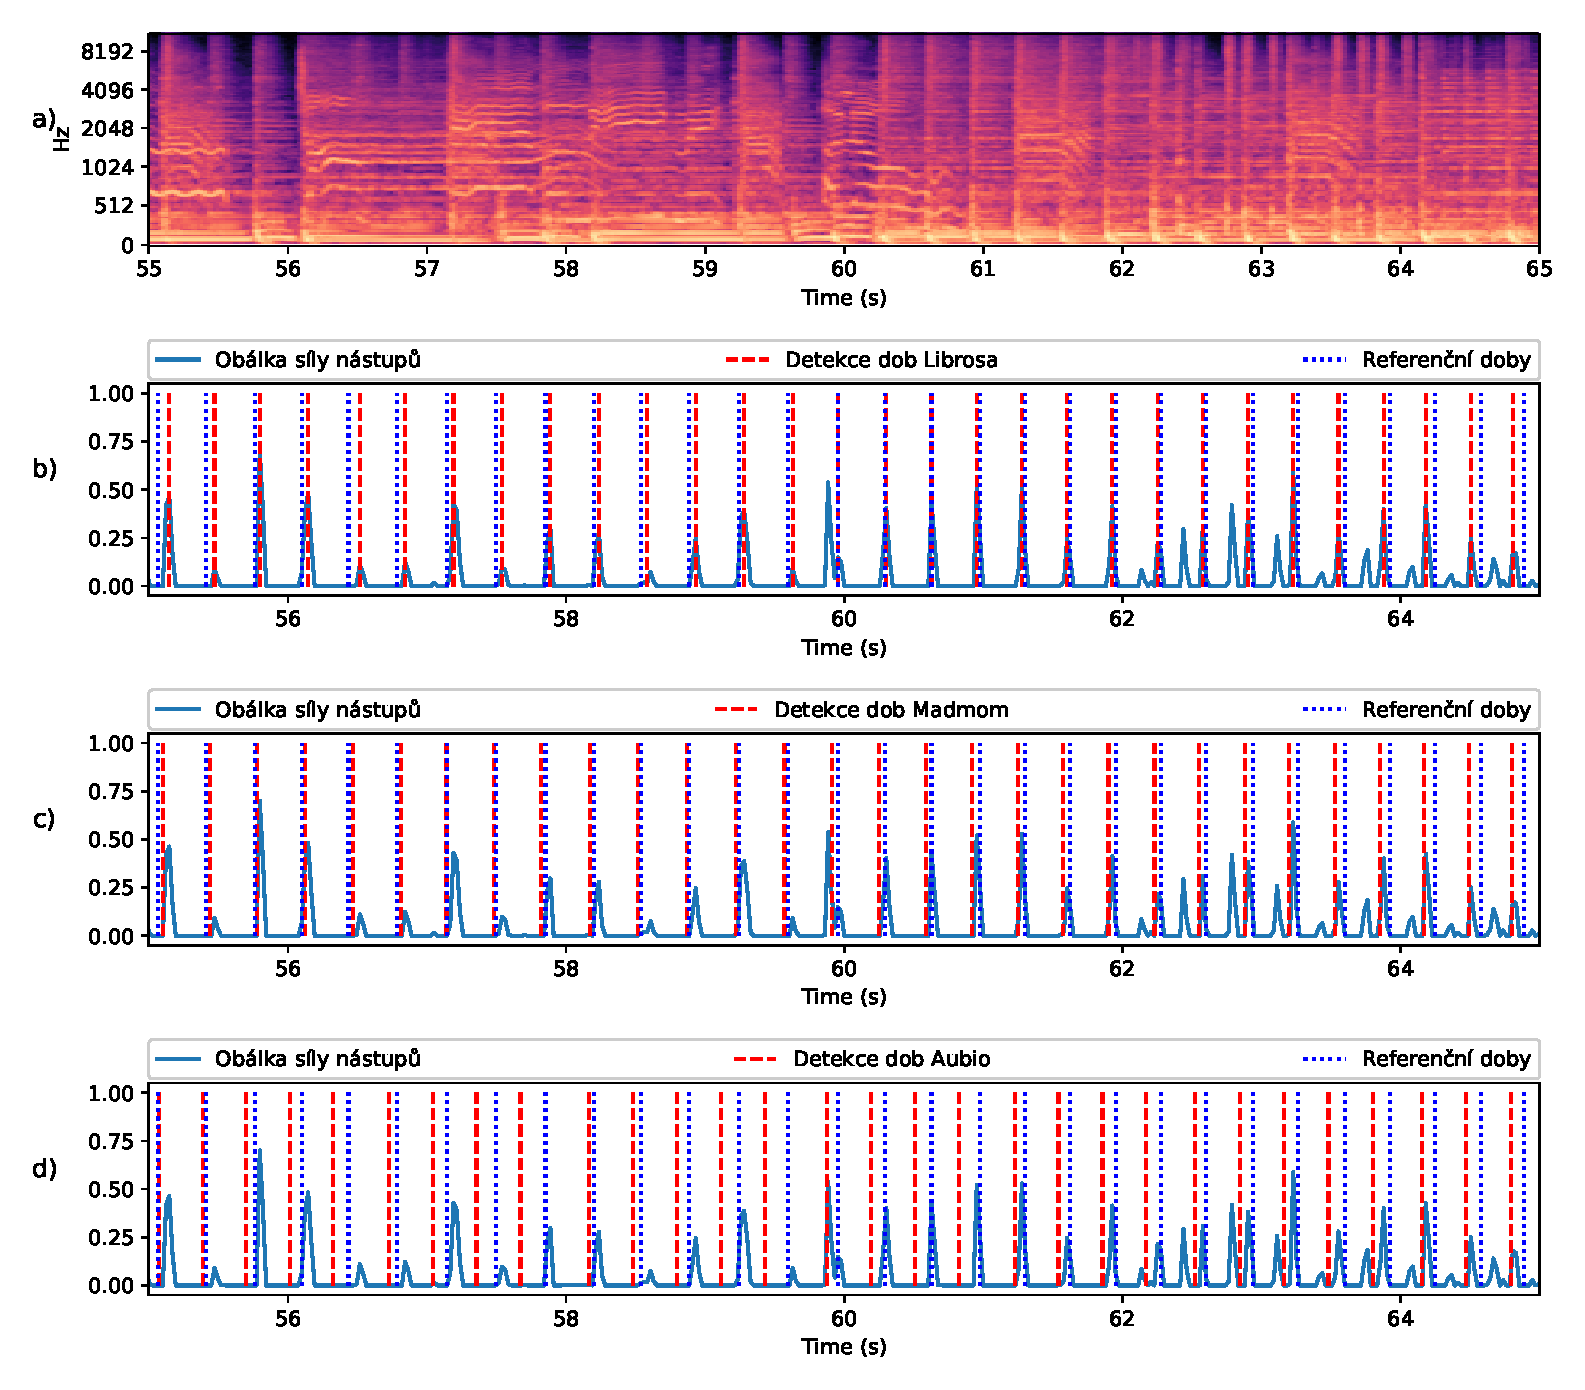
\includegraphics[width = 1\linewidth]{obrazky/Oh-Darling_Beat_analysis_graphs.eps}
    \caption{Porovnání metod detekce dob na úryvku skladby Oh-Darling!. \textbf{a)} Mel spektrogram \textbf{b)}Detekce dob pomocí Librosa \textbf{c)} Detekce dob pomocí Madmom \textbf{d)} Detekce dob pomocí Aubio}
    \label{fig:Oh-Darling_beat_analysis}
\end{figure}

Z grafu lze vidět, že funkce z knihoven Librosa a Madmon se nejvíce přibližují referenčním dobám. Pro přesné hodnocení funkcí je využita knihovna Mir\_eval poskytující funkce pro hodnocení přesnosti detekce dob. Pomocí teto knihovny je počítáno Camgil skóré. Popis knihovny a výpočtu je zmíněn v bodě \ref{sec:Mir_eval}. Posledním hodnoceným parametrem je doba výpočtu. Výsledky Camgil skóré, a doby výpočtu pro jednotlivé skladby jsou zobrazeny na obrázku \ref{fig:Beat_tracking_time_and_cemgil}.

\begin{figure}[H]
    \centering
    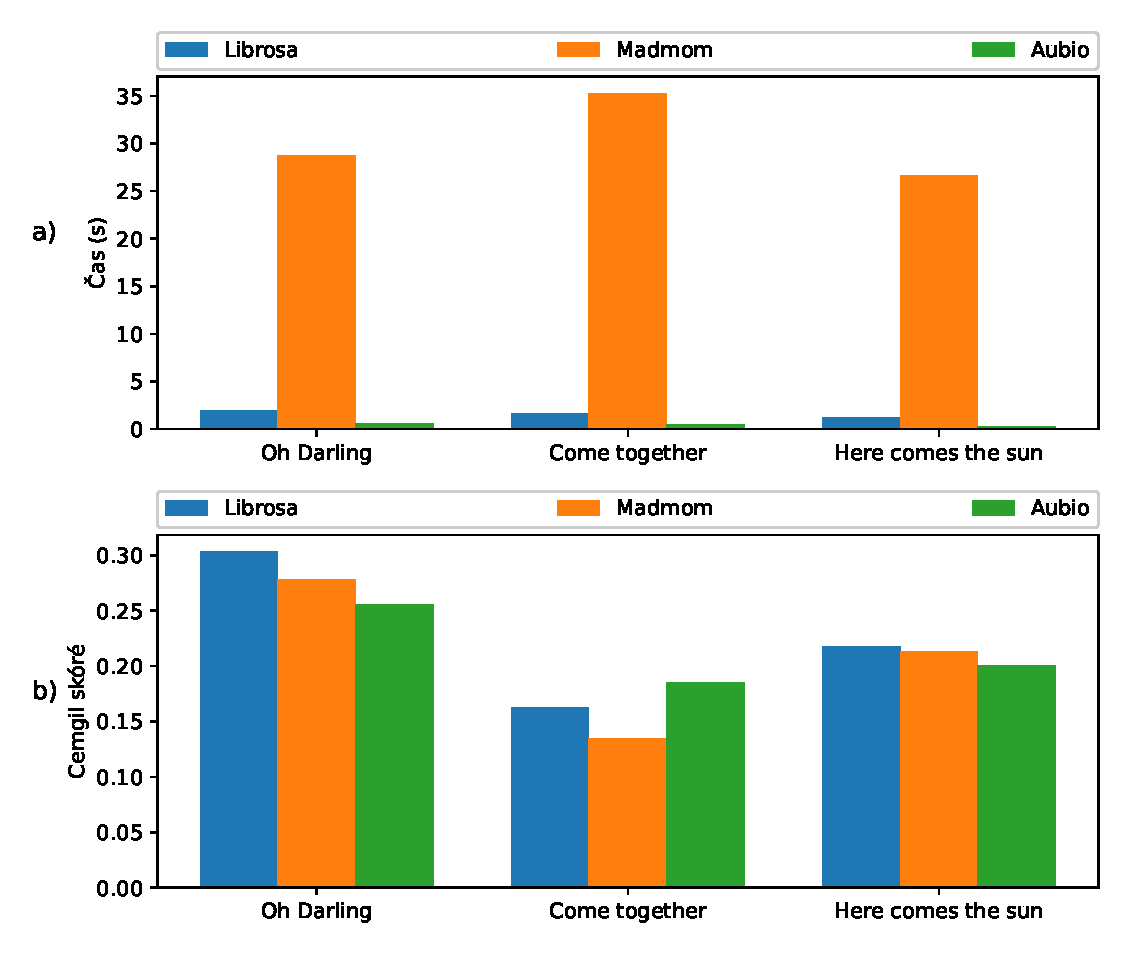
\includegraphics[width = 1\linewidth]{obrazky/Beat_tracking_time_and_cemgil_graphs.eps}
    \caption{Porovnání přesnosti a času metod detekce dob na skladbách Oh-Darling!, Come Together a Here Comes The Sun. \textbf{a)} Čas výpočtu \textbf{b)}Cemgil skóré}
    \label{fig:Beat_tracking_time_and_cemgil}
\end{figure}

\subsection{Analýza chromavektorů}

Hodnocení vhodné funkce pro výpočet chromavektorů je realizováno zejména vizuálně na zobrazených grafech referenčních skladeb. Tyto grafy lze vidět na obrázku \ref{fig:Chroma_analysis}. Porovnávány jsou 4 funkce z knihvny librosa $chroma\_stft$, $chroma\_cqt$, $chroma\_cens$ a čtvrtou je funkce $chroma\_cqt$ c řetězci s předzpracováním signálu a filtrací výsledných chromavektorů. Principy výpočtů jednotlivých funkcí jsou popsány v bodě \ref{sec:Librosa}. Z knihovny Madmom je použit \textit{DeepChromaProcessor}.

\begin{figure}[H]
    \centering
    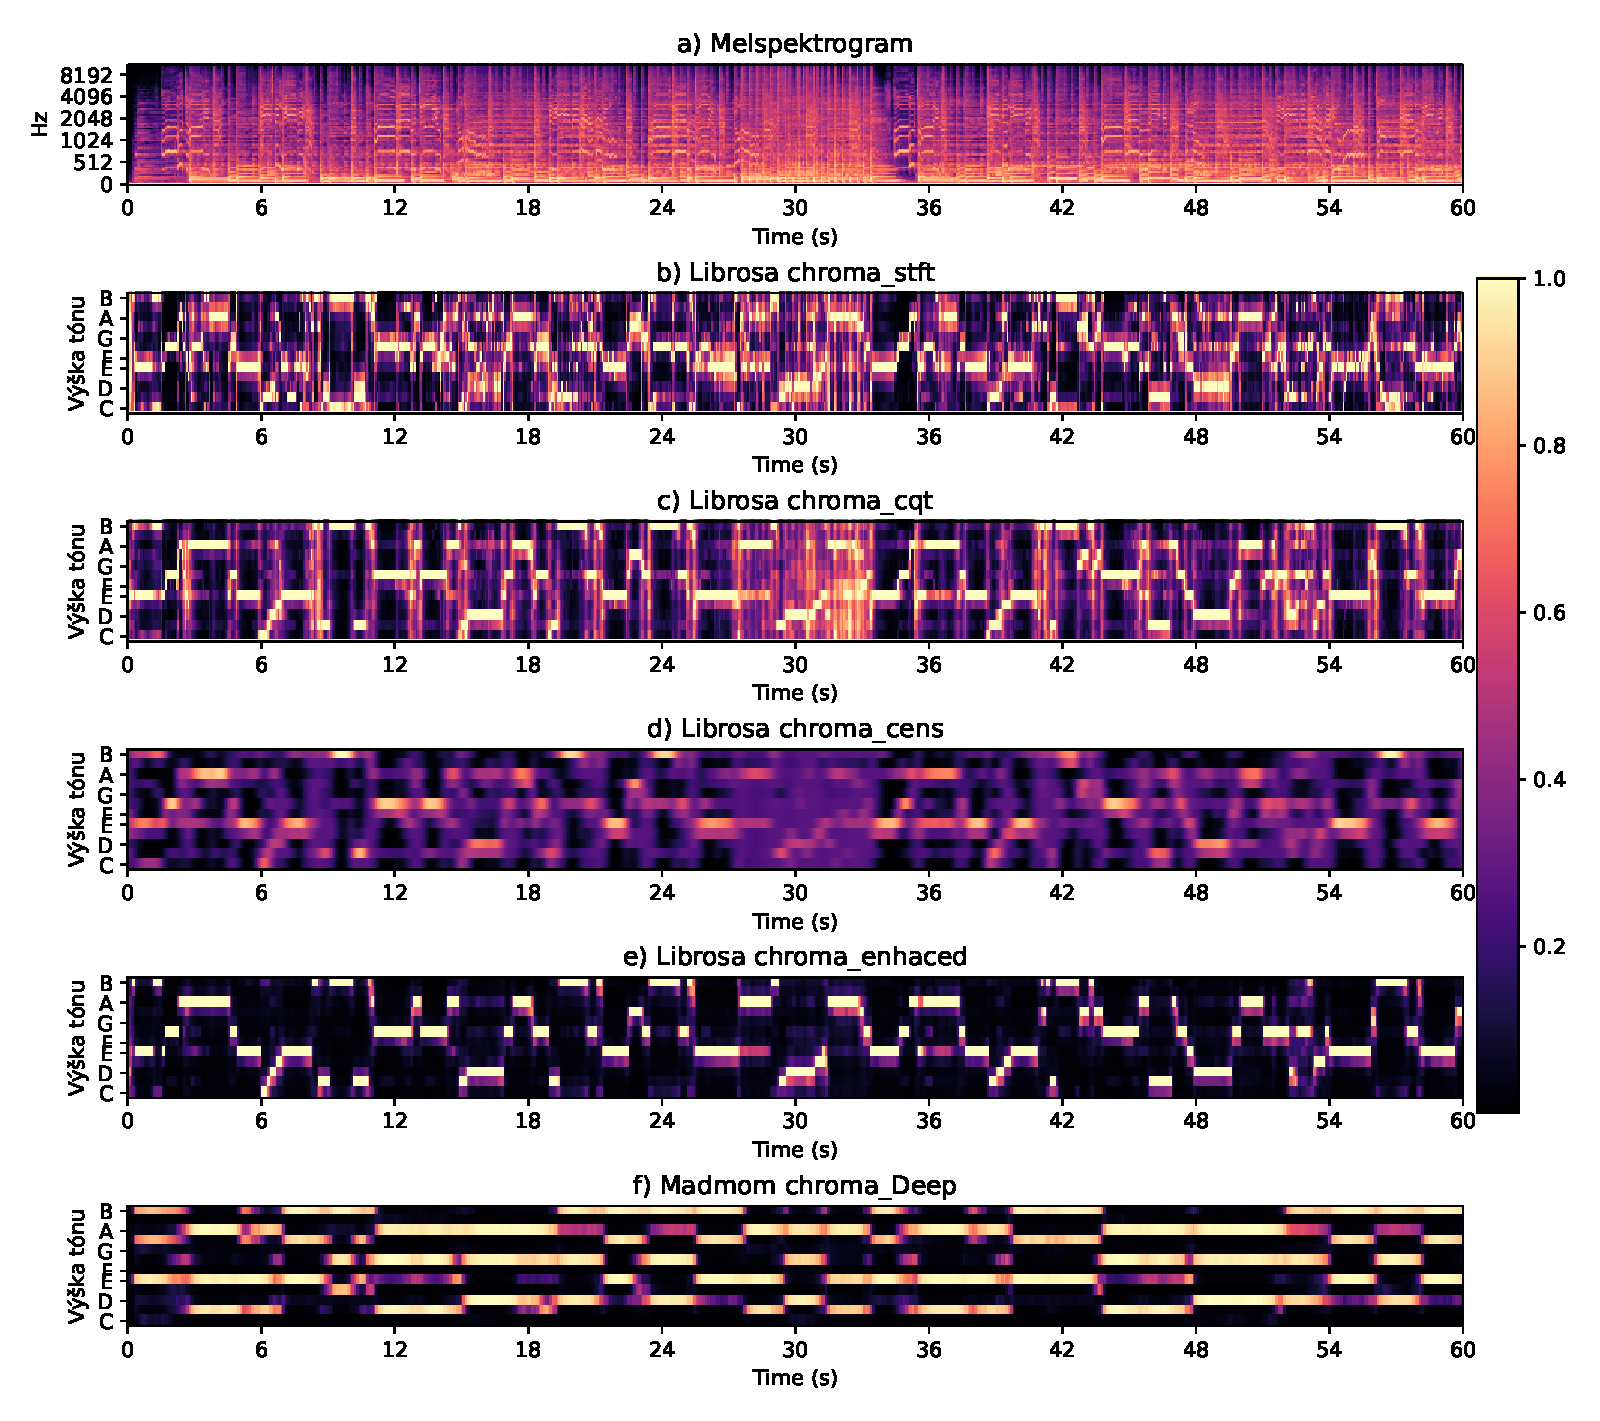
\includegraphics[width = 1\linewidth]{obrazky/Oh-Darling_chroma_analysis_graphs.eps}
    \caption{Porovnání výpočtu chromavektorů na skladbě Oh-Darling! v časovém rozmezí 0 - 60 s.}
    \label{fig:Chroma_analysis}
\end{figure}

Z obrázku \ref{fig:Chroma_analysis} lze vidět patrný rozdíl v přístupu výpočetu chromavektorů. U grafů \textit{b)}, \textit{c)} a \textit{d)} lze vidět velké množství šumu. U grafu \textit{e)} je šum vyfíltrován přidanými metodami. Na grafu \textit{f)} lze vidět, že knihovna Madmom a z ní použitý $DeepChromaProcessor$ přistupuje k výpočtu chromavektorů odlišně. Je využito delší časové okno pro transformaci do frekvenční oblasti. Z toho je patrné, že v časovém měřítku údaj není natolik přesný jako u knihovny Librosa. Pro následné použití v algoritmu pro generování animací je však tento výsledek mnohem stálejší. 

Dalším hodnoceným parametrem je délka výpočtu chromavektorů. Ta je závislá na složitosti algoritmů jež funkce využívají k výpočtu. Porovnání je zobrazeno na obrázku \ref{fig:Chroma_calculation_time}. Z obrázku je zřejmé, že pomocné metody pro předzpracování a filtraci chromavektorů z funkce \textit{chroma\_cqt} přidaly značné množství výpočetního času oproti samotnému výpočtu chromavektorů.

\begin{figure}[H]
    \centering
    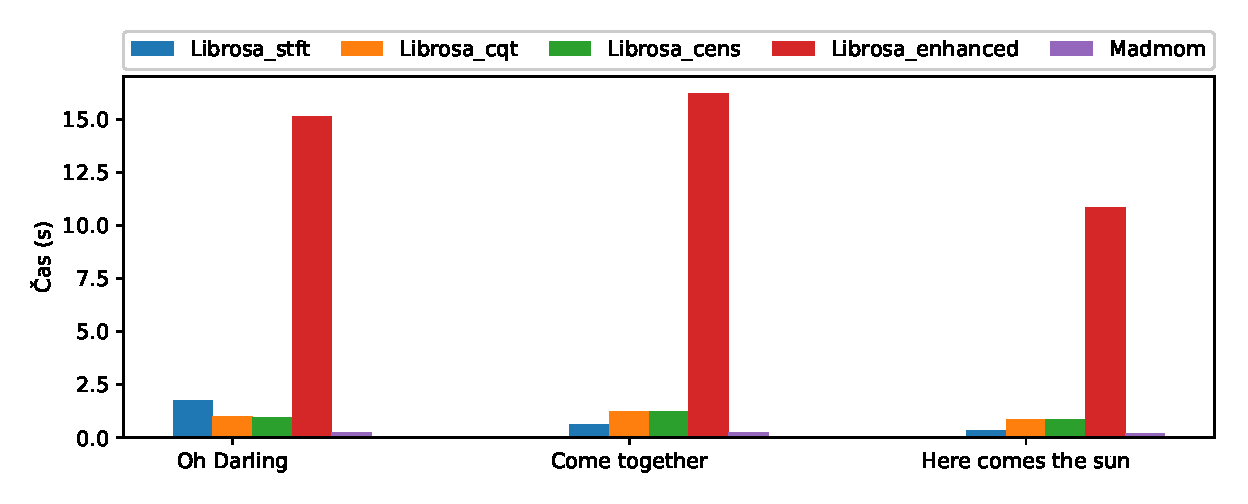
\includegraphics[width = 1\linewidth]{obrazky/Chroma_analysis_times_comparison.eps}
    \caption{Porovnání délky výpočetu chromavektorů}
    \label{fig:Chroma_calculation_time}
\end{figure}

% TODO: Triadické míchání barev v rámci chroma features
    
\subsection{Efektivní hodnota signálu}

Výpočet efektivní hodnoty signálu je raalizován pomocí funkce z knihovy Librosa. Pro výpočet je použito okno o délce 2048 vzorků. Hodnoty jsou vycentrovány na střed rozsahu okna tedy 1024 vzorků. Získaná křivka je uhlazena pomocí výpočtu klouzavého průměru. Počet vzroků ze kterých se klouzavý průměr vypočítá odpovídá délce signálu 7,5 s a je závyslý na jeho vzorkovací frekvenci. Získané informnace jsou zobrazy na obrázku \ref{fig:RMS_calculation}.

\begin{figure}[H]
    \centering
    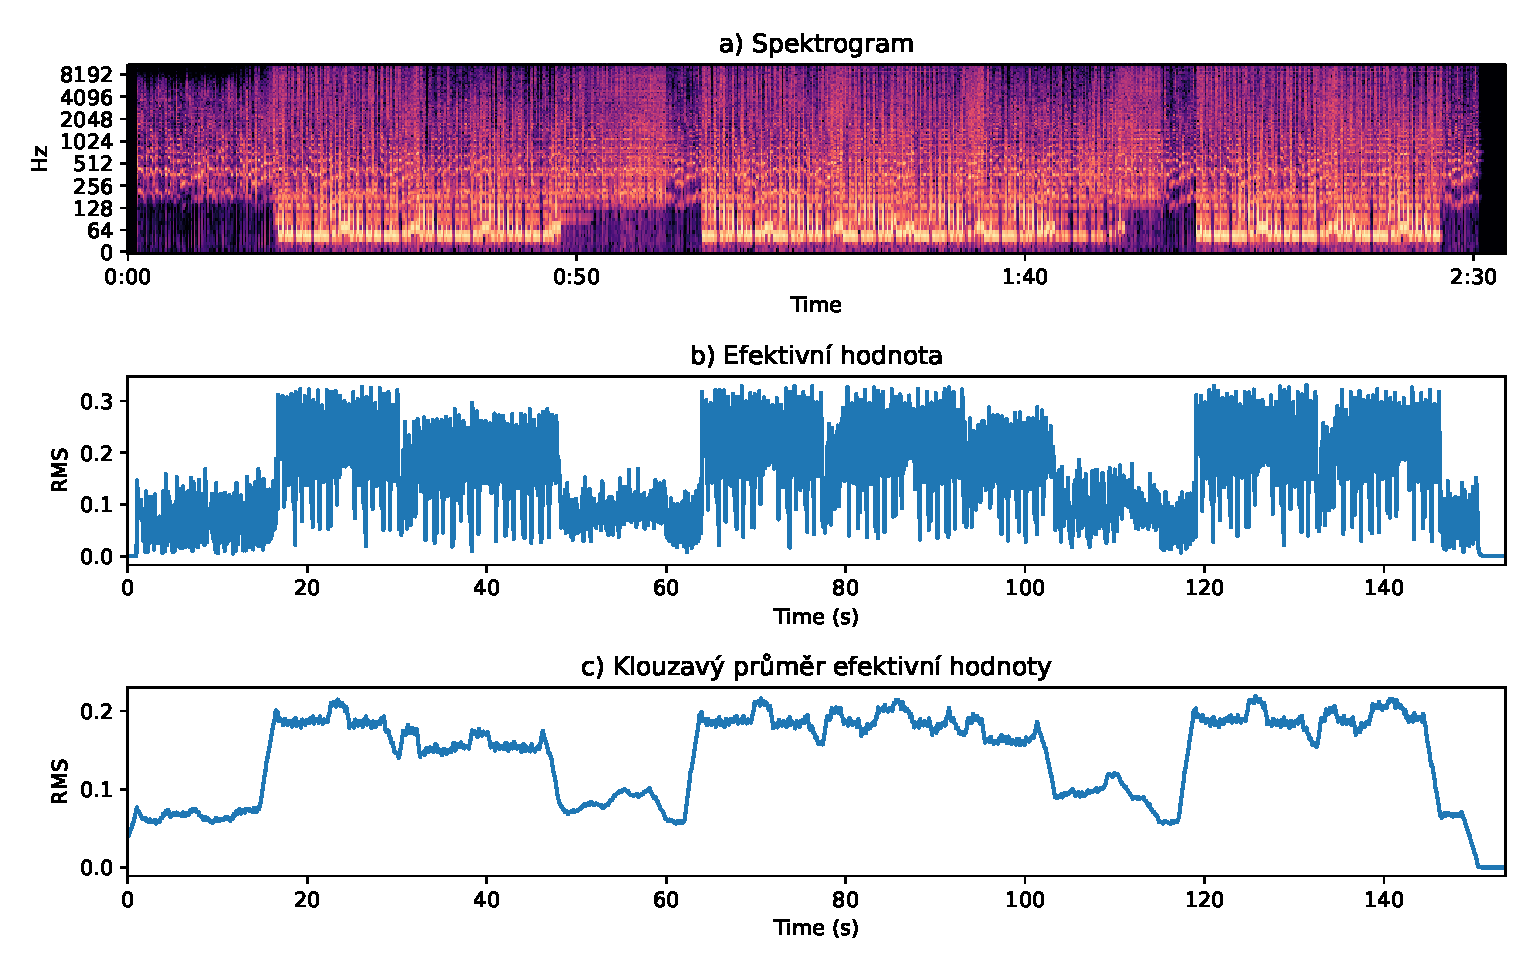
\includegraphics[width = 1\linewidth]{obrazky/Belly_dancer_RMS.eps}
    \caption{Zobrazení efektivní hodnoty skladby Belly dancer}
    \label{fig:RMS_calculation}
\end{figure}

\section{Návrhy na zlepšení}
V této kapitole jsou v odrážkách popsány body a návrehy pro realizaci a zlepšení výsledného systému. 

\begin{itemize}
    \item Prozkoumat oblasti automatické detekce hudebních žánrů a následně realizovat vhodné řešení. Tento parametry je důležitý pro výběr vhodného datasetu. 
    \item Vhodně realizovat segmentaci skladby na jednotlivé části popsané v návrhu segmentace v bodě. \ref{sec:Parametry_nahravky}
    \item Zajímavým bodem pro prozkoumání je porovnání efektivní hodnoty signálu s hlasitostí vypočítanou v jednoce LUFS stanovenou normami EBU R 128 \cite{EBU_R_128}. 
    \item Pro vhodnější výběr bloků animací je možné použít obálku síly nástupů. Na základě které lze určitě sílu daného nástupu a předpokládat významnost doby.
\end{itemize}

% Domyslení procesu přiřazování palety barev a který z chromavektrů bude využit.

